\subsection{Slučaj upotrebe: Upravljanje budžetom i rokovima}

\subsubsection*{Kratak opis}

Producent za projekat animiranog filma postavlja ukupni budžet i planira
budžet i rokove po fazama produkcije (razvoj ideje, scenario, dizajn,
animacija, montaža, postprodukcija, distribucija). Tokom produkcije evidentira
troškove, prati utrošak sredstava i poštovanje rokova, a kada se približi
granici budžeta ili roka, preraspodeljuje sredstva ili menja rok faze.
Projektni menadžer obaveštava se o promenama rokova faza, jer na osnovu njih organizuje produkciju i dodeljuje zadatke.

\subsubsection*{Akteri}
\begin{itemize}
    \item \textbf{Producent} -- postavlja budžet i rokove, evidentira troškove i prati stanje projekta.
    \item \textbf{Projektni menadžer} -- prima obaveštenja o promenama rokova faza i na osnovu njih prilagođava organizaciju produkcije i zadatke.
\end{itemize}

\subsubsection*{Preduslovi}
\begin{itemize}
    \item Producent je prijavljen na sistem i angažovan na projektu.
    \item Projekat animiranog filma postoji u sistemu.
\end{itemize}

\subsubsection*{Postuslovi}
\begin{itemize}
    \item Ukupni budžet, budžet i rokovi faza i evidentirani troškovi su sačuvani u sistemu, a svaka izmena budžeta ili roka zabeležena je sa autorom, datumom i razlogom.
    \item Ako je rok faze promenjen, projektni menadžer je obavešten.
\end{itemize}

\subsubsection*{Osnovni tok}
\begin{enumerate}
    \item Producent bira projekat i opciju ,,Budžet i rokovi''.
    \item Sistem prikazuje pregled faza produkcije sa planiranim budžetom, rokovima i trenutnim utroškom.
    \item Producent bira opciju ,,Planiraj budžet'' i unosi ukupni budžet projekta, kao i za svaku fazu planirani iznos, datum početka i datum završetka.
    \item Sistem proverava podatke i čuva budžet i rokove.
    \item Producent bira opciju ,,Dodaj trošak'' i unosi fazu, iznos, datum i opis troška.
    \item Sistem proverava podatke, evidentira trošak, ažurira utrošak faze i prikazuje preostala sredstva i procenat utroška. Koraci 5 i 6 se ponavljaju kad god nastane novi trošak.
    \item Ako utrošak pređe 80\% budžeta faze ili je rok faze probijen, sistem prikazuje upozorenje i nudi preraspodelu sredstava (podtok P2) ili izmenu roka (podtok P1).
\end{enumerate}

\subsubsection*{Podtokovi}

\paragraph*{P1: Izmena roka faze}
\begin{enumerate}
    \item Producent u pregledu faza bira fazu i opciju ,,Izmeni rok''.
    \item Producent unosi novi datum početka i/ili završetka i razlog izmene.
    \item Sistem proverava da novi rok ne dolazi u sukob sa fazama koje zavise od izabrane faze, čuva izmenu i obaveštava projektnog menadžera.
\end{enumerate}

\paragraph*{P2: Preraspodela sredstava između faza}
\begin{enumerate}
    \item Producent bira opciju ,,Preraspodeli sredstva''.
    \item Producent bira fazu iz koje se sredstva prenose, fazu u koju se prenose i iznos, unosi razlog i potvrđuje.
    \item Sistem proverava da budžet faze izvora ne padne ispod već utrošenog iznosa, ažurira budžete obe faze i beleži izmenu. Ukupni budžet projekta ostaje isti.
\end{enumerate}

\paragraph*{P3: Pregled stanja budžeta i rokova}
\begin{enumerate}
    \item Producent bira opciju ,,Stanje budžeta i rokova''.
    \item Sistem prikazuje za svaku fazu planirani budžet, utrošena sredstva, preostali iznos, odstupanje od plana i status roka (u roku, kasni, završena).
    \item Producent po želji filtrira prikaz po fazi ili vremenskom periodu.
\end{enumerate}

\subsubsection*{Alternativni tokovi}

\paragraph*{A1: Nepopunjena ili neispravna polja}
\begin{itemize}
    \item U koracima 4 i 6 osnovnog toka, kao i u koracima 3 podtoka P1 i P2, ako neko obavezno polje nije popunjeno ili je neispravno (datum završetka pre datuma početka, zbir budžeta faza veći od ukupnog budžeta), sistem ga označava i vraća producenta na unos.
\end{itemize}

\paragraph*{A2: Budžet je već postavljen}
\begin{itemize}
    \item U koraku 3 osnovnog toka, ako projekat već ima budžet, sistem prikazuje postojeće vrednosti za izmenu umesto praznog unosa; izmena se čuva uz razlog.
\end{itemize}

\paragraph*{A3: Prekoračenje budžeta faze}
\begin{itemize}
    \item U koraku 6 osnovnog toka, ako bi trošak premašio preostala sredstva faze, sistem upozorava producenta i nudi preraspodelu sredstava (podtok P2) ili evidentiranje troška uz obavezno obrazloženje.
\end{itemize}

\paragraph*{A4: Probijen rok faze}
\begin{itemize}
    \item U koraku 7 osnovnog toka i u podtoku P3, ako je datum završetka faze prošao, a faza nije završena, sistem je označava kao ,,kasni'' i nudi izmenu roka (podtok P1).
\end{itemize}

\paragraph*{A5: Odustajanje}
\begin{itemize}
    \item U bilo kom koraku producent može da odustane; sistem ne čuva nesačuvane izmene i vraća ga na stranicu projekta.
\end{itemize}

\subsubsection*{Specijalni zahtevi}
\begin{itemize}
    \item Evidentirani troškovi se ne brišu; greška se ispravlja novim, korektivnim unosom.
    \item Budžet faze ne sme se smanjiti ispod već utrošenog iznosa, a zbir budžeta faza ne sme preći ukupni budžet.
    \item Faza koja ima evidentirane troškove ne sme se obrisati bez upozorenja.
\end{itemize}

\subsubsection*{Dodatne informacije}
\begin{itemize}
    \item Pregled izveštaja o realizaciji projekata je zaseban slučaj upotrebe.
\end{itemize}


\begin{figure}[H]
	\centering
	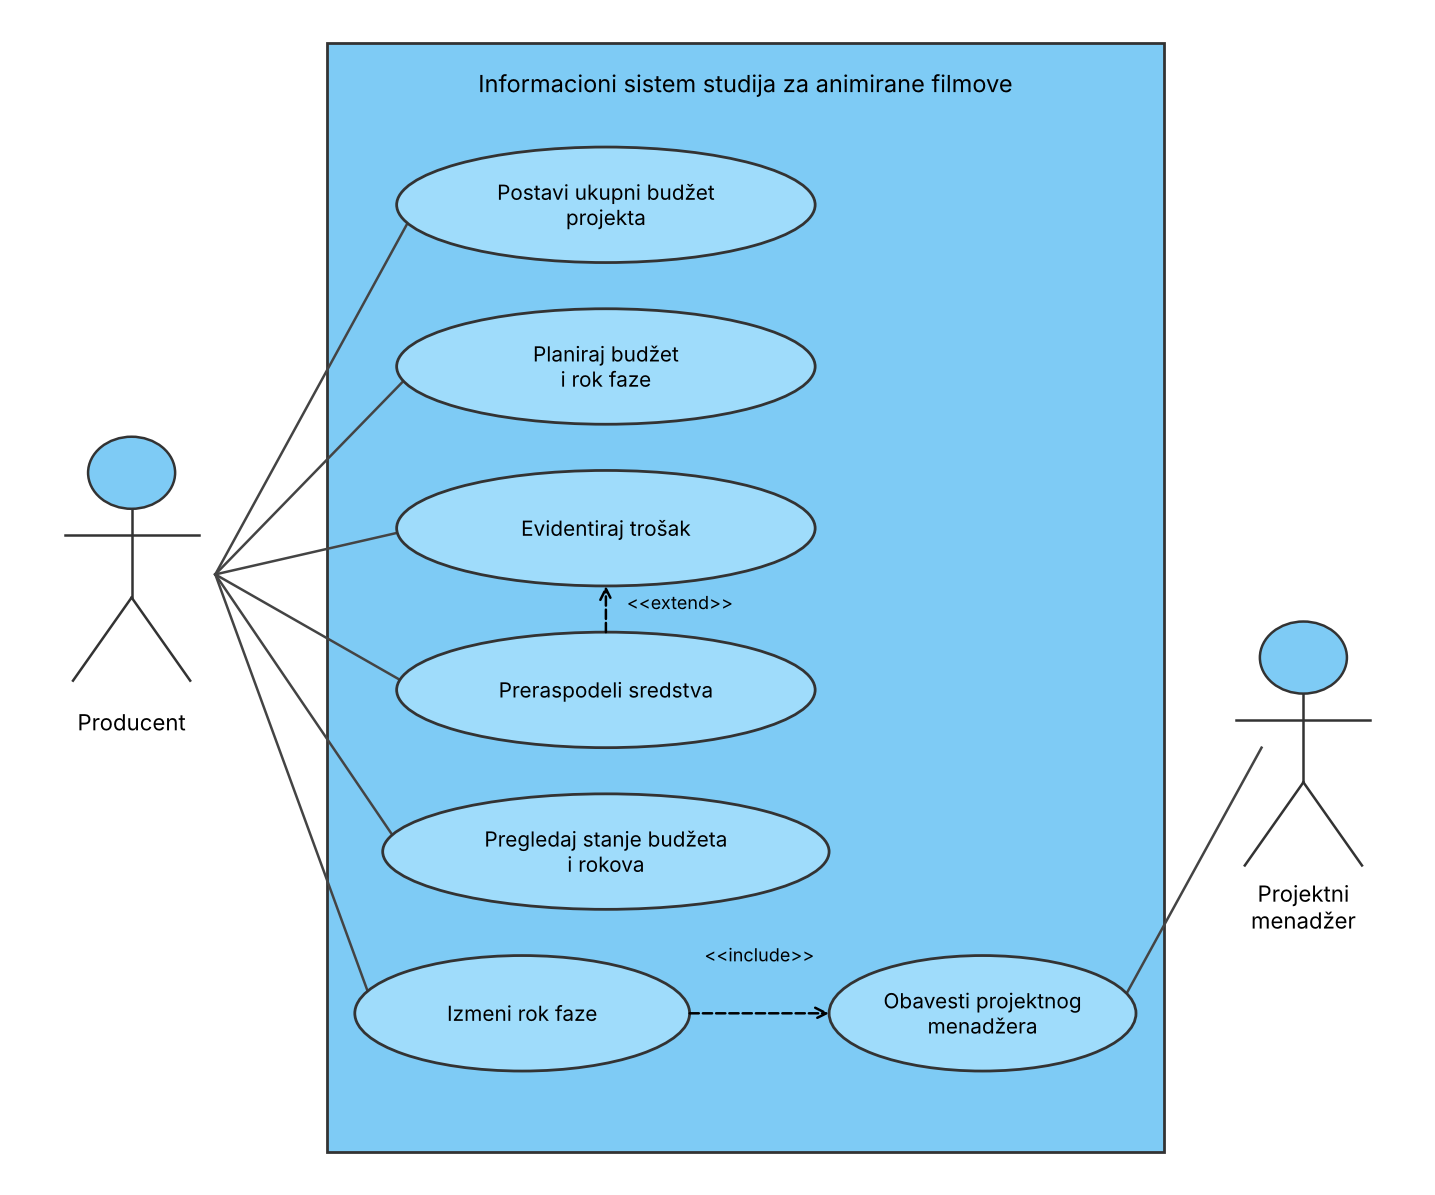
\includegraphics[width=\textwidth]{./dijagrami/dijagrami_slucajeva_upotrebe/upravljanje_budzetom_i_rokovima.png}
	\caption{Dijagram slučaja upotrebe ,,Upravljanje budžetom i rokovima''}
 \end{figure}

\begin{figure}[H]
	\centering
	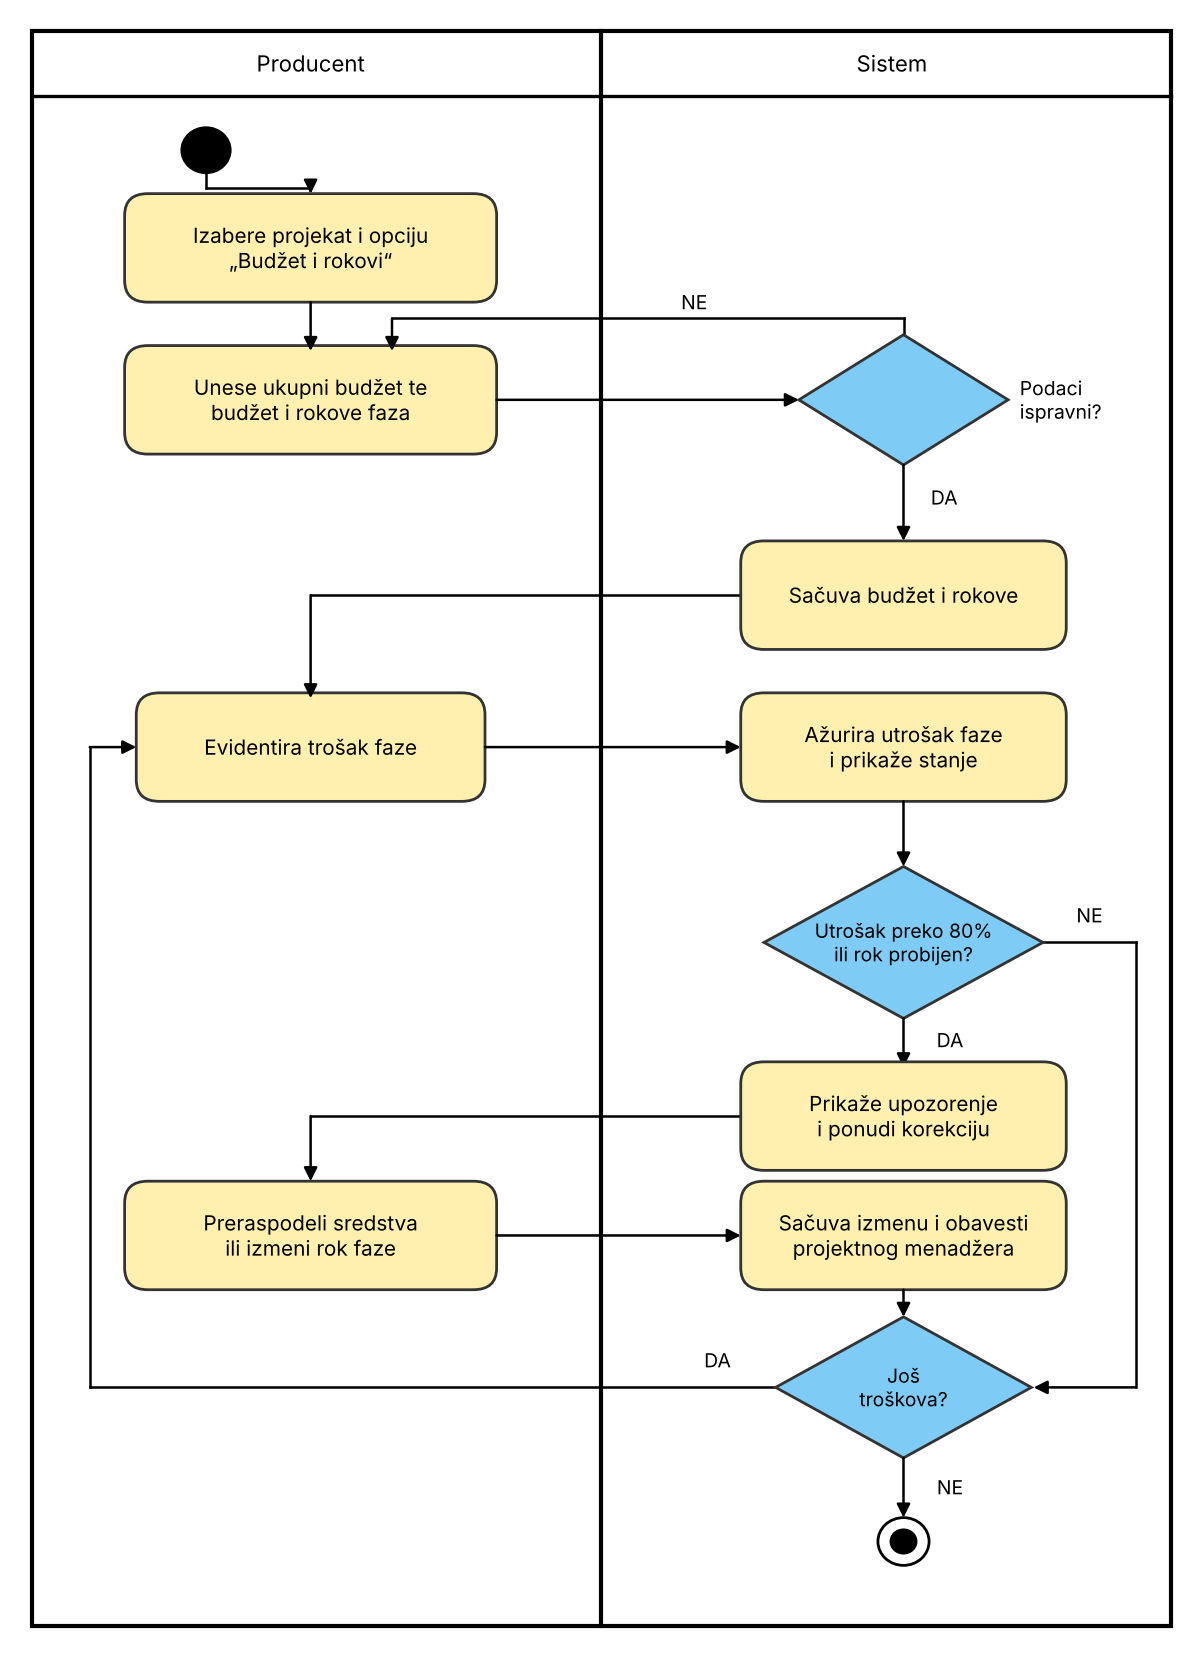
\includegraphics[width=\textwidth,height=0.8\textheight,keepaspectratio]{./dijagrami/dijagrami_aktivnosti/upravljanje_budzetom_i_rokovima.png}
	\caption{Dijagram aktivnosti ,,Upravljanje budžetom i rokovima''}
 \end{figure}

\begin{figure}[H]
	\centering
	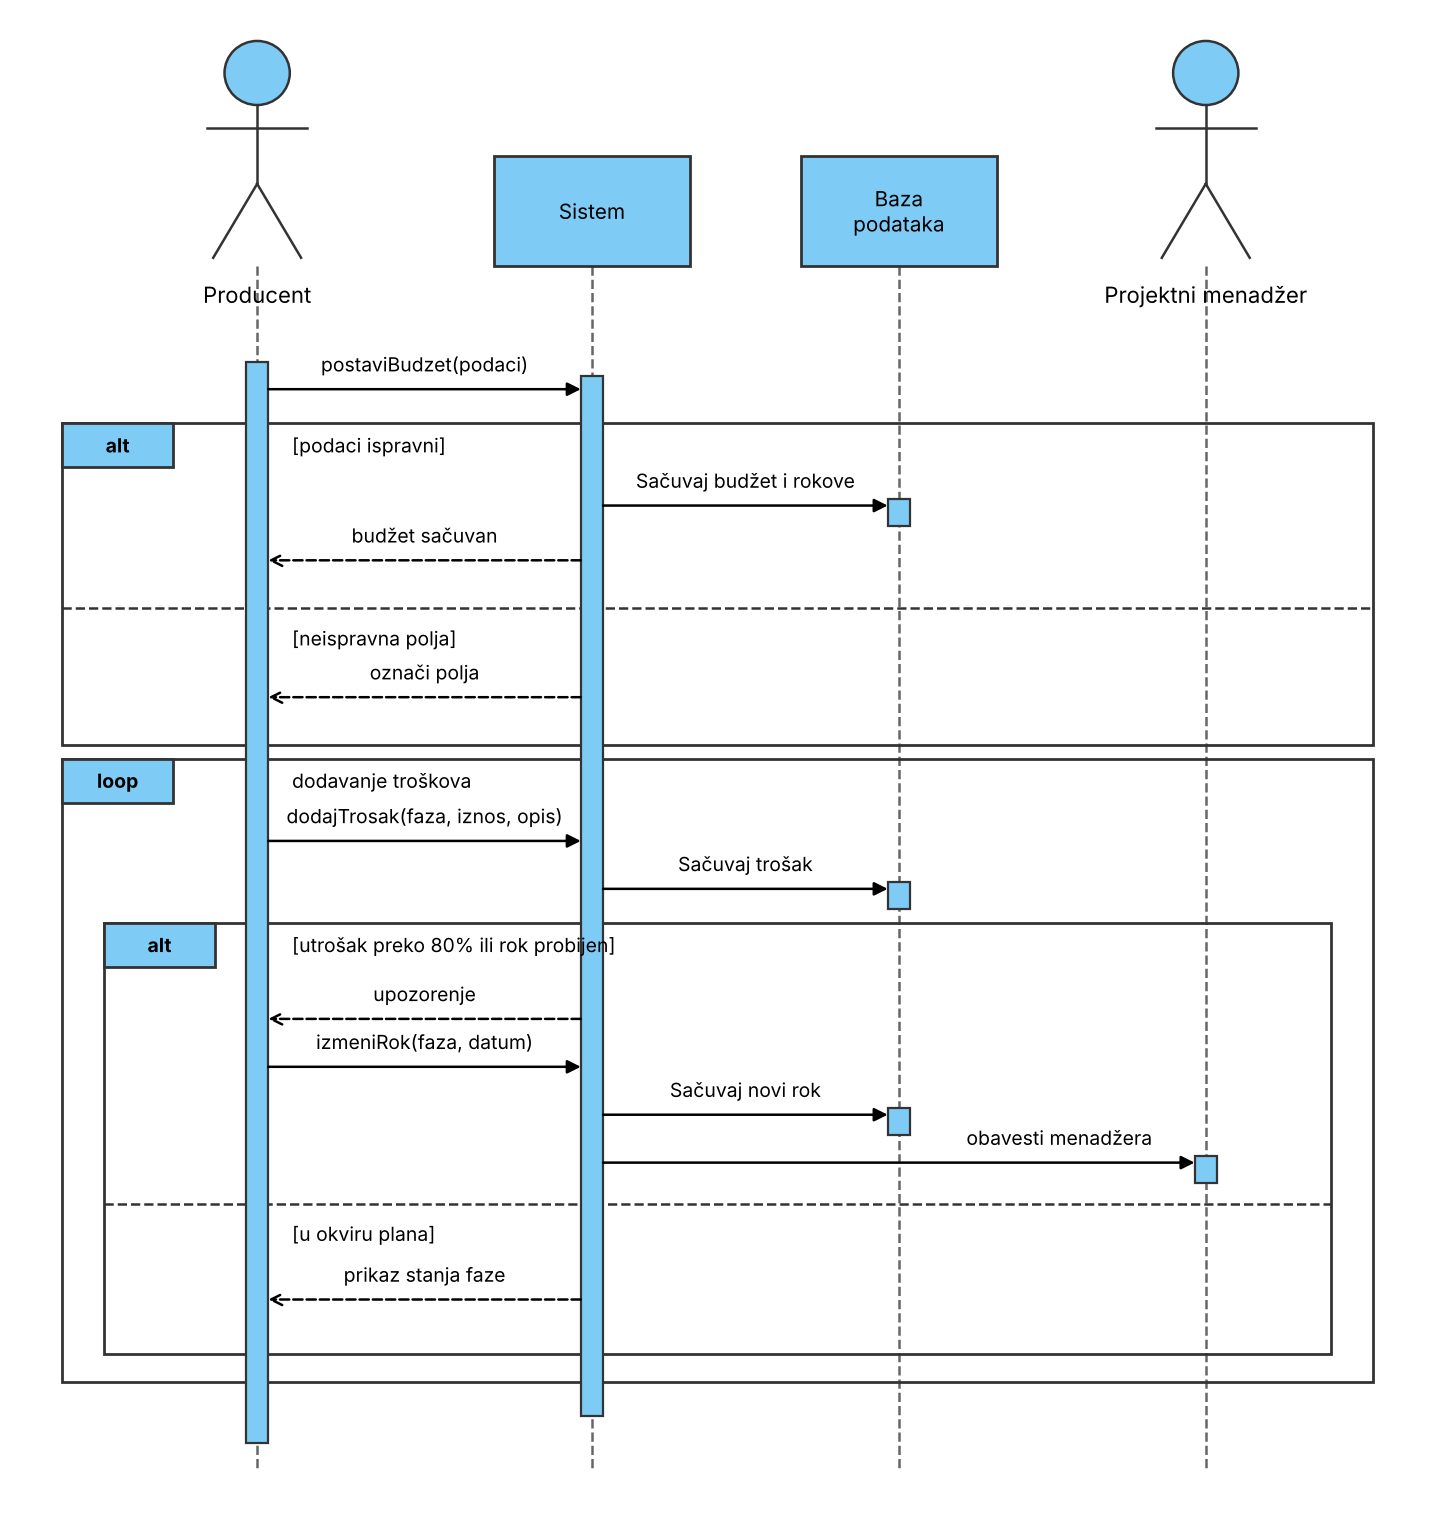
\includegraphics[width=\textwidth]{./dijagrami/dijagrami_sekvence/upravljanje_budzetom_i_rokovima.png}
	\caption{Dijagram sekvence ,,Upravljanje budžetom i rokovima''}
 \end{figure}

\newpage
